\documentclass[11pt, oneside]{article} 
\usepackage{geometry}
\geometry{letterpaper} 
\usepackage{graphicx}
	
\usepackage{amssymb}
\usepackage{amsmath}
\usepackage{parskip}
\usepackage{color}
\usepackage{hyperref}

\graphicspath{{/Users/telliott_admin/Dropbox/Tex/png/}}
% \begin{center} 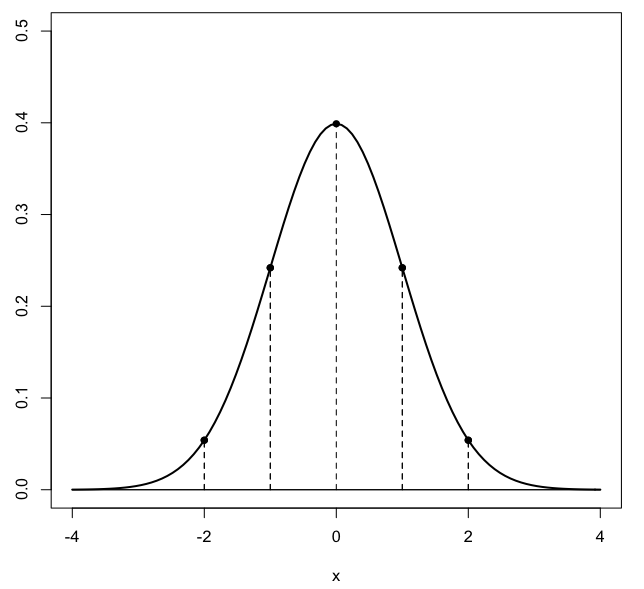
\includegraphics [scale=0.4] {gauss3.png} \end{center}

\title{Completeness}
\date{}

\begin{document}
\maketitle
\Large

The property of completeness distinguishes the set of real numbers $\mathbb{R}$ from the rationals  $\mathbb{Q}$.

One informal statement of completeness is that "the real number line has no holes in it."  In contrast, the set of rational numbers is missing the irrationals such as $\sqrt{2}$ and $e$ and so on.

\subsection*{bounds}

Suppose $\mathbf{A}$ is a non-empty subset of $\mathbb{R}$, then an upper bound of $\mathbf{A}$ is an element $b \in \mathbb{R}$ such that $b \ge a$ for all $a \in \mathbf{A}$.

$\circ$  Example:  suppose $\mathbf{A}$ consists of all $x \in \mathbb{R} \ | \ x < 0$.  Then $100$ is an upper bound for $\mathbf{A}$, and so is $1$ and so is $0$.

The reason for the restriction to non-empty subsets has to do with the definition of an upper bound.  The statement $b > a$ for every member $a \in \mathbf{A}$ is \emph{true} if  $\mathbf{A}$ is empty ($\mathbf{A} = \varnothing$).

\subsection*{least upper bound}

$\bullet$  $u$ is an upper bound for $\mathbf{A}$ if $\forall \ x \in \mathbf{A}, x \le u$

$\bullet$  $U$ least upper bound for $\mathbf{A}$ if for all upper bounds $u$, $U \le u$

Note that for $U = sup(\mathbf{A}$) it is not necessary that $U \in \mathbf{A}$.

$\circ$  Example:  suppose $\mathbf{A}$ consists of all $x \in \mathbb{R} \ | \ x < 0$.  Then $0$ is the least upper bound of $\mathbf{A}$.

$0$ is the least upper bound of both $\{x \ | \ x < 0\}$ and $\{x \ | \ x \le 0\}$, but only in the second case is $0$ a member of the set.

The least upper bound of a subset of $\mathbb{R}$ is often called the \textbf{supremum} of the set, as in $\mathbf{sup}(\mathbf{A}) = 0$.  The supremum is not necessarily $\in \mathbf{A}$, but if it is then it is the maximum element of $\mathbf{A}$.

\subsection*{completeness axiom}

$\bullet$  Every non-empty subset of $\mathbb{R}$ that is bounded above has a supremum in $\mathbb{R}$.

If a non-empty set $\mathbf{A}$ has an upper bound, it has a least upper bound.

This is not a true statement for $\mathbb{Q}$.  Suppose we define the subset of $\mathbb{Q}$ that contains all numbers $r \ | \ r^2 < 2$.  Then, $\sqrt{2}$ is the supremum of this set, but $\sqrt{2} \notin \mathbb{Q}$.

\subsection*{approximation property}

Apostol gives this corollary to the completeness axiom:  

Let $\mathbf{S}$ be a non-empty set of real numbers with a supremum, say $b = sup(\mathbf{S}$).  Then for every $a < b$ there is some $x$ in $\mathbf{S}$ such that
\[ a < x \le b \]

\textbf{Proof}:  

First, $x \le b$ for all x in $\mathbf{S}$.  If we had $x \le a$ for all $x$ in $\mathbf{S}$, then $a$ would be an upper bound for $\mathbf{S}$ smaller than the least upper bound.  Therefore, $x > a$ for at least one $x$ in $\mathbf{S}$.

An epsilon-delta definition says:  if $\mathbf{A}$ is bounded above with $u = sup \ \mathbf{A}$ then
\[ \forall \ \epsilon > 0 \ \exists \ x_{\epsilon} \in  \mathbf{A} \ | \  x_{\epsilon} > u - \epsilon \]

There is no "last number" before the least upper bound.  No matter how small you make $\epsilon$, one can always find $x$ whose distance from $u$ is smaller than $\epsilon$.

No matter how small is $\epsilon$ we can always find a negative number closer to zero than that.

\end{document}}